\documentclass{standalone}
\usepackage{pgfplots}
\pgfplotsset{compat=newest}

\begin{document}
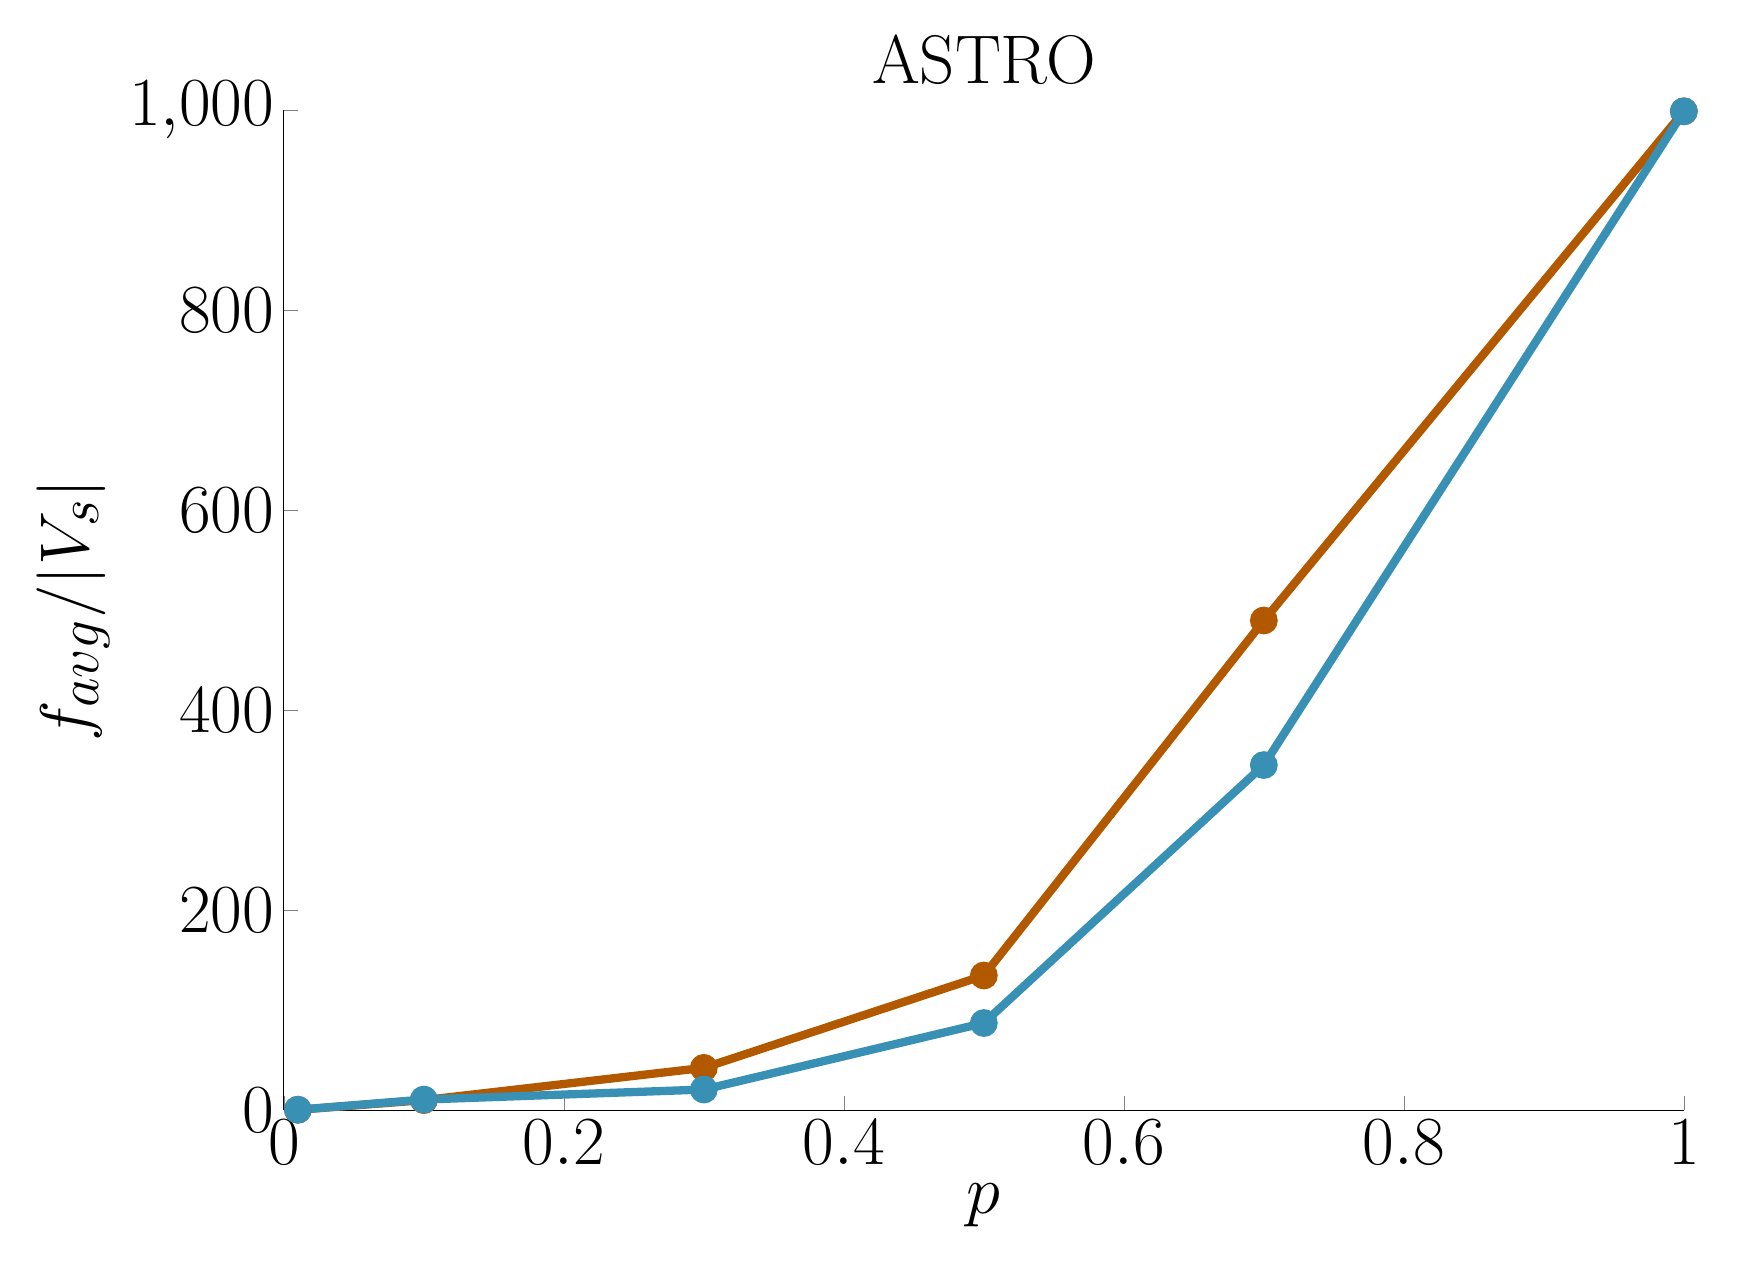
\begin{tikzpicture}

\begin{axis}[%
title style={font=\Huge},
title=ASTRO,
tick label style={font=\Huge},
label style={font=\Huge},
legend style={font=\Huge},
view={0}{90},
width=7in,
height=5in,
scale only axis,
xmin=0, xmax=1,
xtick={0, 0.2, 0.4, 0.6, 0.8, 1},
xlabel={$p$},
ymin=0, ymax=1000,
ytick={0, 200, 400, 600, 800, 1000},
ylabel={$f_{avg} / |V_s|$},
major tick length=5pt,
axis lines*=left,
legend cell align=left,
clip=false]

\addplot [
mark=*,
mark size=3.5pt,
color=orange!70!black,
solid,
line width=3pt
]
coordinates{
(0.01,0.5312)(0.1,10.1848)(0.3,42.469)(0.5,134.777142857)(0.7,489.82)(1,999.0)
};

\addplot [
mark=*,
mark size=3.5pt,
color=cyan!70!black,
solid,
line width=3pt
]
coordinates{
(0.01,0.6084)(0.1,10.7644)(0.3,20.7759661099)(0.5,87.282636664)(0.7,345.253809524)(1,999.0)
};

\end{axis}
\end{tikzpicture}
\end{document}
